\documentclass[10pt]{extarticle}

%SOME USEFUL PACKAGES
\usepackage[portuguese]{babel}
\usepackage{extsizes}
\usepackage[reqno]{amsmath} % equation numbers on the right
\usepackage{amsmath}
\usepackage{amssymb}
\usepackage{amsthm}
\usepackage{amscd}
\usepackage{indentfirst}
\usepackage{amsfonts}
\usepackage{listings}
\usepackage{graphicx}
\usepackage{dsfont}
\usepackage{fancyhdr}
\usepackage{enumerate}
\usepackage[utf8]{inputenc}
\usepackage{booktabs}
\usepackage{listings}
\usepackage[margin=1in]{geometry}
\usepackage[hypcap]{caption}
\usepackage{longtable}
\usepackage{etoolbox}
%\usepackage[alf]{abntex2cite}
\usepackage[siunitx]{circuitikz}
\usepackage{tikz}
\usepackage{enumitem}
\usepackage{algorithm}
\usepackage{algorithmic}


\usepackage{verbatim}
\usepackage{float}
\usepackage{xcolor}

\definecolor{codegreen}{rgb}{0,0.6,0}
\definecolor{codegray}{rgb}{0.5,0.5,0.5}
\definecolor{codepurple}{rgb}{0.58,0,0.82}
\definecolor{backcolour}{rgb}{1, 1, 1}

\lstdefinestyle{mystyle}{
    backgroundcolor=\color{backcolour},   
    commentstyle=\color{codegreen},
    keywordstyle=\color{magenta},
    numberstyle=\tiny\color{codegray},
    stringstyle=\color{codepurple},
    basicstyle=\ttfamily\footnotesize,
    breakatwhitespace=false,         
    breaklines=true,                 
    captionpos=b,                    
    keepspaces=true,                 
    numbers=left,                    
    numbersep=5pt,                  
    showspaces=false,                
    showstringspaces=false,
    showtabs=false,                  
    tabsize=2
}

\lstset{style=mystyle}
%HEADER
\pagestyle{fancy}\lhead{B. Poggiali -- V. Julião Ramos} \rhead{DCC023 - Redes de Computadores - 2020.1}
\chead{{\large{\bf }}} \lfoot{} \rfoot{\bf \thepage} 
\cfoot{}


\title{ \textsc{Universidade Federal de Minas Gerais} \\ \textsc{Departamento de Ciência da Computação} \\ \bigskip TP3 -- DCC-RIP}

\author{Breno Poggiali de Sousa \\ \normalsize{brenopoggiali@gmail.com}\\
Vinicius Julião Ramos \\ \normalsize{viniciusjuliao@dcc.ufmg.br}}

\date{\today}

\begin{document}
\maketitle

\begin{abstract}
    O trabalho aqui desenvolvido consiste na construção de um modelo virtual
    para um roteador que implementar o protocolo RIP.
    Nessa aplicação, o algoritmo de \textit{Distance Vector} foi introduzido e
    através de um código encapsulado com a função apenas de gerênciar a tabela
    de roteamento.
    Esse encapsulamento, permitiu que cada uma das funções solicitadas pela
    especificação do trabalho fossem desenvolvidas de forma independente.
    Tais funções são: Atualizações periódicas, \textit{Split
    Horizon}, rerroteamento imediato e a remoção de rotas desatualizadas.
\end{abstract}

\section{Introdução}

Para possibilitar a virtualização de um roteador, através de um aplicação,
necessitou-se utilizar um protocolo da camada de transporte.
Nesse cenário, optou-se pelo UDP, uma vez que esse protocolo é o que mais se
aproxima da camada de rede, pelo motivo de não fornecer quaisquer garantias
de entrega, controle de erros ou gerenciamento de conexão.
Portanto, para esse socket, uma classe \textbf{Router} foi criada com a
finalidade de gerenciar a troca de informações.
Essa mesma classe é responsável por executar comandos em duas \textit{thread}
diferentes, sendo que uma delas recebe comandos da entrada padrão do sistema e 
a outra executa o protocolo de rede especificado pelo trabalho.

A opção de criar uma classe separada para gerenciar a tabela de roteamento
permitiu gerênciar todas a funções que cabem à uma tabela de roteamento: a
remoção de rotas desatualizadas, a montagem da lista de distâncias através
do \textit{Split Horizon} e também o rerroteamente imediato. Essa última função
é desempenhada por demanda, o que permite que a melhor rota para determinado
endereço seja calculada apenas quando o roteador envia mensagem para tal
destino. Já a atualização periódica de rotas é uma atividade conjunta entre o
roteador e a tabela de roteamento; a tabela de roteamento entrega ao roteador
a lista de distâncias, mas cabe ao roteador atualizar os vizinhos de acordo com
o período especificado.
\section{Decisões de Implementação}
\begin{figure}[h]
	\begin{center}
		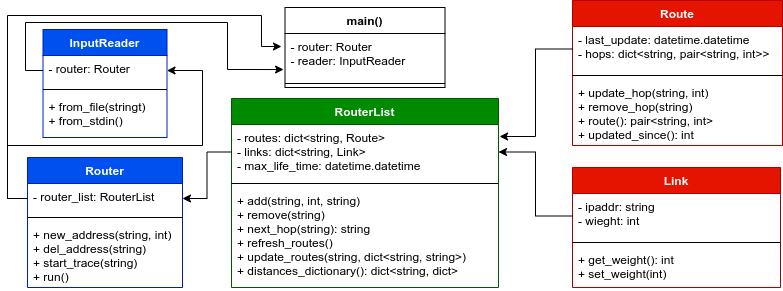
\includegraphics[scale=0.55]{fig/uml.png}
	\end{center}
	\caption{\label{fig:digrama} Diagrama da estrutura de classes.}
\end{figure}

Essa seção trata de como as quatro principais funções, requeridas pela descrição
do trabalho, foram desenvolvidas.
Também é colocado em cheque as dificuldades referentes às soluções propostas.
Mas antes de descrever a implementação, é necessário abordar três estruturas de
dados presentes na classe RouterList:
\begin{itemize}
    \item \textbf{Route}: Atributo \textbf{ipaddr}: é o endereço final da rota.
    Atributo \textbf{last\_update}: é um atributo que salva a ultima vez em que
    a rota foi atualizada.
    Atributo \textbf{hops}: é um dicionário \textbf{(K\_addr, V)} em que
    \textbf{K\_addr} é o endereço ip do link associado ao roteador e \textbf{V}
    é o custo de enviar uma mensagem para o endereço \textbf{ipaddr} passando pelo
    link \textbf{K\_addr}.
    \item \textbf{RouterList.\_\_routes}: Trata-se de um dicionário
    \textbf{(R\_addr, R)}. Nesse caso \textbf{R\_addr} é o endereço de uma
    máquina e \textbf{R} trata-se da instância de \textbf{Route} correspondente
    a tal destino.
    \item \textbf{RouterList.\_\_links}: Dicionário \textbf{(L\_addr, L)} em
    que os links de endereço \textbf{L\_addr} são informados na entrada padrão,
    através do comando \texttt{add}, juntamente com o seu peso.
    Essa informação é armazenada em uma instãncia da classe \textbf{Link}.
\end{itemize}


\subsection{Atualizações Periódicas}
A cada meio segundo, é feito uma chamada ao método \texttt{Router.\_\_share\_router\_list}.
Então esse método trata de analisar se já passou tempo suficiente desde a
última atualização, para que uma nova atualização seja feita.
Caso seja necessário atualizar novamente, então as listas de distâncias 
são requisitados da tabela de roteamento.
Como essa lista de distâncias pode variar de acordo com o link, devido ao
\textit{Split Horizon}, o retorno dessa chamada é um dicionário, em que cada
elemento \textbf{(addr, dist)} corresponde à chave \textbf{addr} (endereço) do
link e \textbf{dist} é a respectiva lista de distancias.

O método itera sobre o dicionário e envia uma mensagem de \texttt{update}
contendo a respectiva lista de distâncias de cada um dos vizinhos.
Observe que o método recebe um atributo \textbf{past}, que é um
\texttt{datetime} da ultima vez em que uma atualização foi enviada.
Caso uma atualização seja feita, então retorno \texttt{True} informa que o
atributo \textbf{past} deve ser atualizado para o momento corrente.

\lstinputlisting[language=Python,
label=code:share-router-list,
caption=Envio das atualizações periódicas das listas de roteamento]
{codes/share_routes.py}

\subsection{Remoção de rotas desatualizadas}
Essa funcionalidade é desempenhada pela classe \textbf{RouterList}.
Como tal classe é a única que possui o controle para inserção, remoção e
atualização das rotas, é natural que esses trabalho seja executado pela tabela
de roteamento.
Ao instanciar um objeto \textbf{RouterList}, deve-se informar qual o tempo de
vida de uma rota desatualizada.
Isso serve para que cada rota criada, tenha um \textit{timer} associado, e esse
contador de tempo consiga analisar se o tempo de vida foi extrapolado ou não.
Observe que objetos \textbf{Route} implementa seu próprio \textit{timer} pelo
atributo \textbf{last\_update}.

O período de remoção das rotas desatualizadas é igual a $4 \times period$, em
que $period$ é o tempo de atualização das rotas dos links vizinhos.
Como no método \texttt{\_\_share\_router\_list} há um controle sobre $period$,
optou-se por implementar uma chamada ao método \texttt{RouterList.refresh\_routes}
no mesmo controlador do envio das listas de distâncias; assim como mostra a
Linha 7 do Listing \ref{code:share-router-list}.
Sendo assim, a cada $period$ segundos, valisa-se se há rotas desatualizadas.
Isso se dá pelo seguinte código:
\lstinputlisting[language=Python,
label=code:refresh-routes,
caption=Remoção das rotas desatualizadas]
{codes/refresh_routes.py}

Há outro fator que merece atenção: Quando uma mensagem do tipo \texttt{update}
chega até o roteador, então a tabela de rotas deve ser atualizada.
Nessa atualização da tabela de rotas, todas aquelas rotas contidas na mensagem
têm seu \textit{timer} atualizado para o momento corrente.
Isso faz com que essa rota ganhe mais tempo de vida.

\subsection{Rerroteamento imediato}
É importante ressaltar que todo roteamento executado pelo servidor é feito de
forma imediata.
Ou seja, a melhor rota para determinado destino é calculada apenas quando uma
mensagem for enviada para tal endereço.
A troca de mensagens é desempenhada pela classe \textbf{Router}, sendo que
qualquer envio de dados é executado pelo método \texttt{Router.\_\_send\_message\_as\_json}. 
Observando o Listing \ref{code:route}, a cadeia de chamadas que retorna a melhor
rota inicia-se na Linha 16, em que o endereço de destino é informado para
\texttt{Router.next\_hop}.
Nesse ultimo método, caso não haja uma rota para tal endereço, então um valor
\texttt{None} é retornado, mas caso contrário, requisita-se o cálculo da rota
para classe \textbf{Route}.
Por fim, \texttt{Route.route} retorna o endereço da rota que possui menor peso.

\lstinputlisting[language=Python,
label=code:route,
caption=Retorna a melhor rota]
{codes/route.py}

Na abordagem aplicada para esse calculo de rerroteamento mesmo quando uma rota
é removida ou alterada da tabela de roteamento, as demais rotas permanecem
intactas.
Logo, para o caso em que a melhor rota para um endereço $X$ fora removida,
quando \textbf{Router} desejar enviar outra mensagem para $X$, uma nova melhor
rota será obtida pela chamada de \texttt{RouterList.next\_hop(X)}

\subsection{Spilt Horizon}
O método \textit{Split Horizon} é aplicado na geração dos dicionários
\textit{distances} que posteriormente serão adicionados às mensagens.
Antes de gerar o dicionário \textbf{distances} que associa o endereço do
vizinho à sua lista de distâncias, gera-se um dicionário contendo todas as
melhores rotas (\textbf{all\_distances}).
Então, para gerar \textbf{distances[link]} -- que é o dicionário de distâncias
de determinado link -- itera-se sobre todos os vizinhos, de forma que
\textbf{distances[link]} recebe todas as rotas que obedecem à optimização
\textit{Split Horizon}.
Ou seja, \textbf{distences[link]} recebe um dicionário contendo as rotas as
quais o endereço de \textbf{link} não seja dado como o melhor caminho.

\lstinputlisting[language=Python,
label=code:all-distances,
caption=Retorna o dicionário de distâncias usando Split Horizon]
{codes/split_horizon.py}



\section{Conclusão}
O trabalho prático foi útil para entender como um roteador realiza seu trabalho.
Usando a abordagem de do protocolo RIP, pode-se entender a importância da
decisão e a escolha entre as rotas e quão isso é importante.
Além disso, é válido ressaltar que o algoritmo que implementa uma tabela de
roteamento usando o algoritmo de Vetor de Distâncias foi implementado na classe
\textbf{RouteList}, entretanto, caso seja necessário mudar o algoritmo de roteamento,
basta substituir tal classe.
\end{document}